
\documentclass{article}
% Comment the following line to NOT allow the usage of umlauts
\usepackage[utf8]{inputenc}
\usepackage[pdftex]{graphicx}
% Uncomment the following line to allow the usage of graphics (.png, .jpg)
%\usepackage{graphicx}

% Start the document
\begin{document}
\section {mendetory part}
student id = 20152424
name = Rocky Kim
github address = https://github.com/Epicevent/assignment01.git
\section{How to use Git}

git is version control software.
you can make new gitproject.
 follow up.
first, login to github.com
second, create new project and install git.exe.
well done ! if you do well
the homepage looks like this fig.
\begin{figure}
\centering
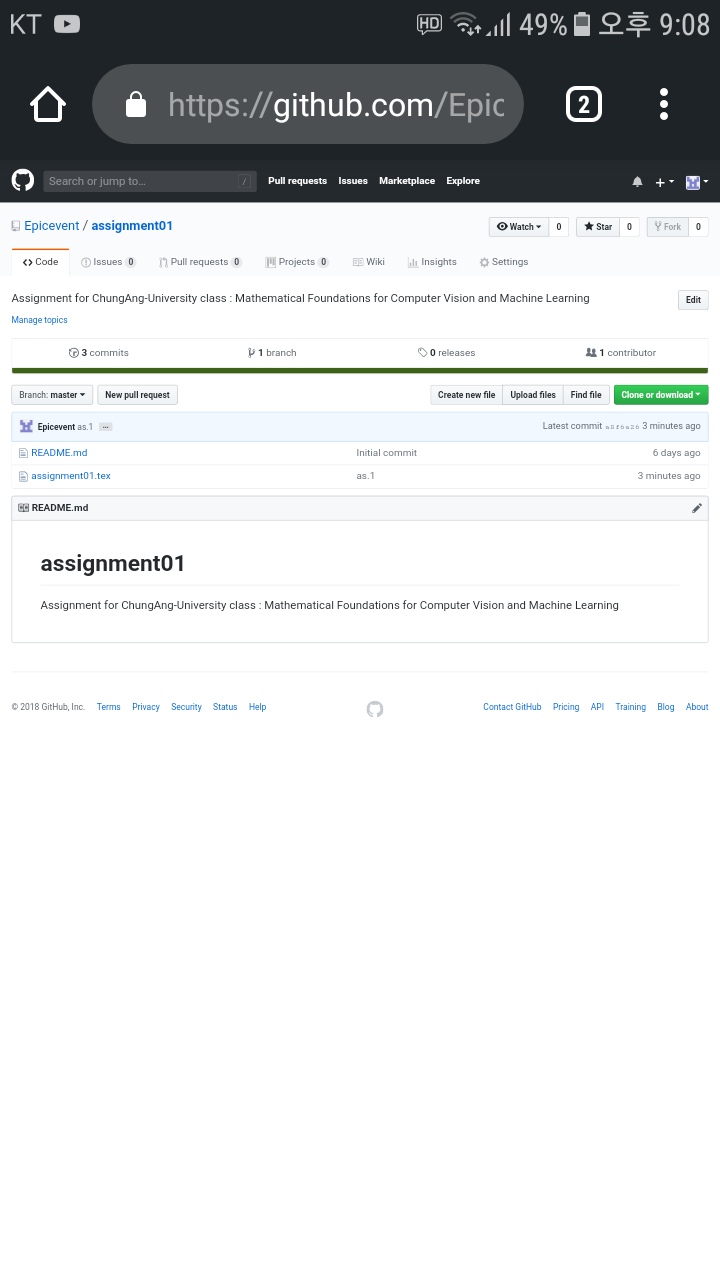
\includegraphics[width=0.4\textwidth]{1537445777178}
\caption{caption}
\end{figure}
\section{Push and commit}
Connect Your Local Repository To Your GitHub Repository

Having a local repository as well as a remote (online) repository is the best of both worlds. You can tinker all you like without even being connected to the Internet, and at the same time showcase your finished work on GitHub for all to see.



% Uncomment the following two lines if you want to have a bibliography
%\bibliographystyle{alpha}
%\bibliography{document}

\end{document}
